\documentclass[12pt]{article}

\usepackage{graphicx}
\usepackage{listings}
\usepackage{hyperref}
\usepackage{float}
\usepackage{enumitem}

\graphicspath{ {./images/} }

\oddsidemargin 0mm
\evensidemargin 0mm
\textwidth 160mm
\textheight 200mm

\pagestyle {plain}
\pagenumbering{arabic}

\newcounter{stepnum}

\title{CS/SE 2XC3 Lab 10 Report}
\author{
  Glotov, Oleg\\ L03, 400174037\\
  \texttt{glotovo@mcmaster.ca}
  \and
  Willson, Emma\\ L02, 400309856\\
  \texttt{willsone@mcmaster.ca}
  }
\date{\today}

\begin{document}

\maketitle

This report includes the main observations that we found in this week's lab, along with the analysis of our results.

\newpage 
\section{Shortest Path}
In this section, we discuss algorithms for finding the shortest path in directed weighted graphs, potentially with negative edge weights. 
\subsection{Bellman-Ford Approximation}
In this implementation of the Bellman-Ford algorithm, there is an array of counters that keeps track of how many times the line \verb-dist[neighbour] = dist[node] + G.w(node, neighbour)- is run on each node. When the count for a node surpasses the input value $k$, the algorithm stops updating the shortest distance to that node.\\
We tested our approximation of Bellman-Ford using connected graphs of size $n=100$ (where $n$ is the number of nodes) with edge weights randomly chosen between 1 and 1000.
The testing method used was consistent with earlier labs. We used \verb+create_random_connected_graph()+ to generate a random graph given a number of nodes and maximum edge weight. We ran the original \verb+bellman_ford()+ and our \verb+bellman_ford_approximation()+ on each graph using $k$ values ranging from 1 to 40. For each $k$ value, each algorithm was tested three times on three different graphs. When testing, we recorded the runtime for each algorithm and the calculated total distance to every other node. Each data point is the average of these three trials. \\
We expect our approximation algorithm to perform better than the original Bellman-Ford algorithm for low values of $k$ because $k$ puts a ceiling on the number of times the distance to a node can be updated. This is one of the most expensive aspects of the algorithm, so capping it should allow it to terminate sooner. The performance of both algorithms is shown in the chart below.
\begin{figure}[H]
\centering
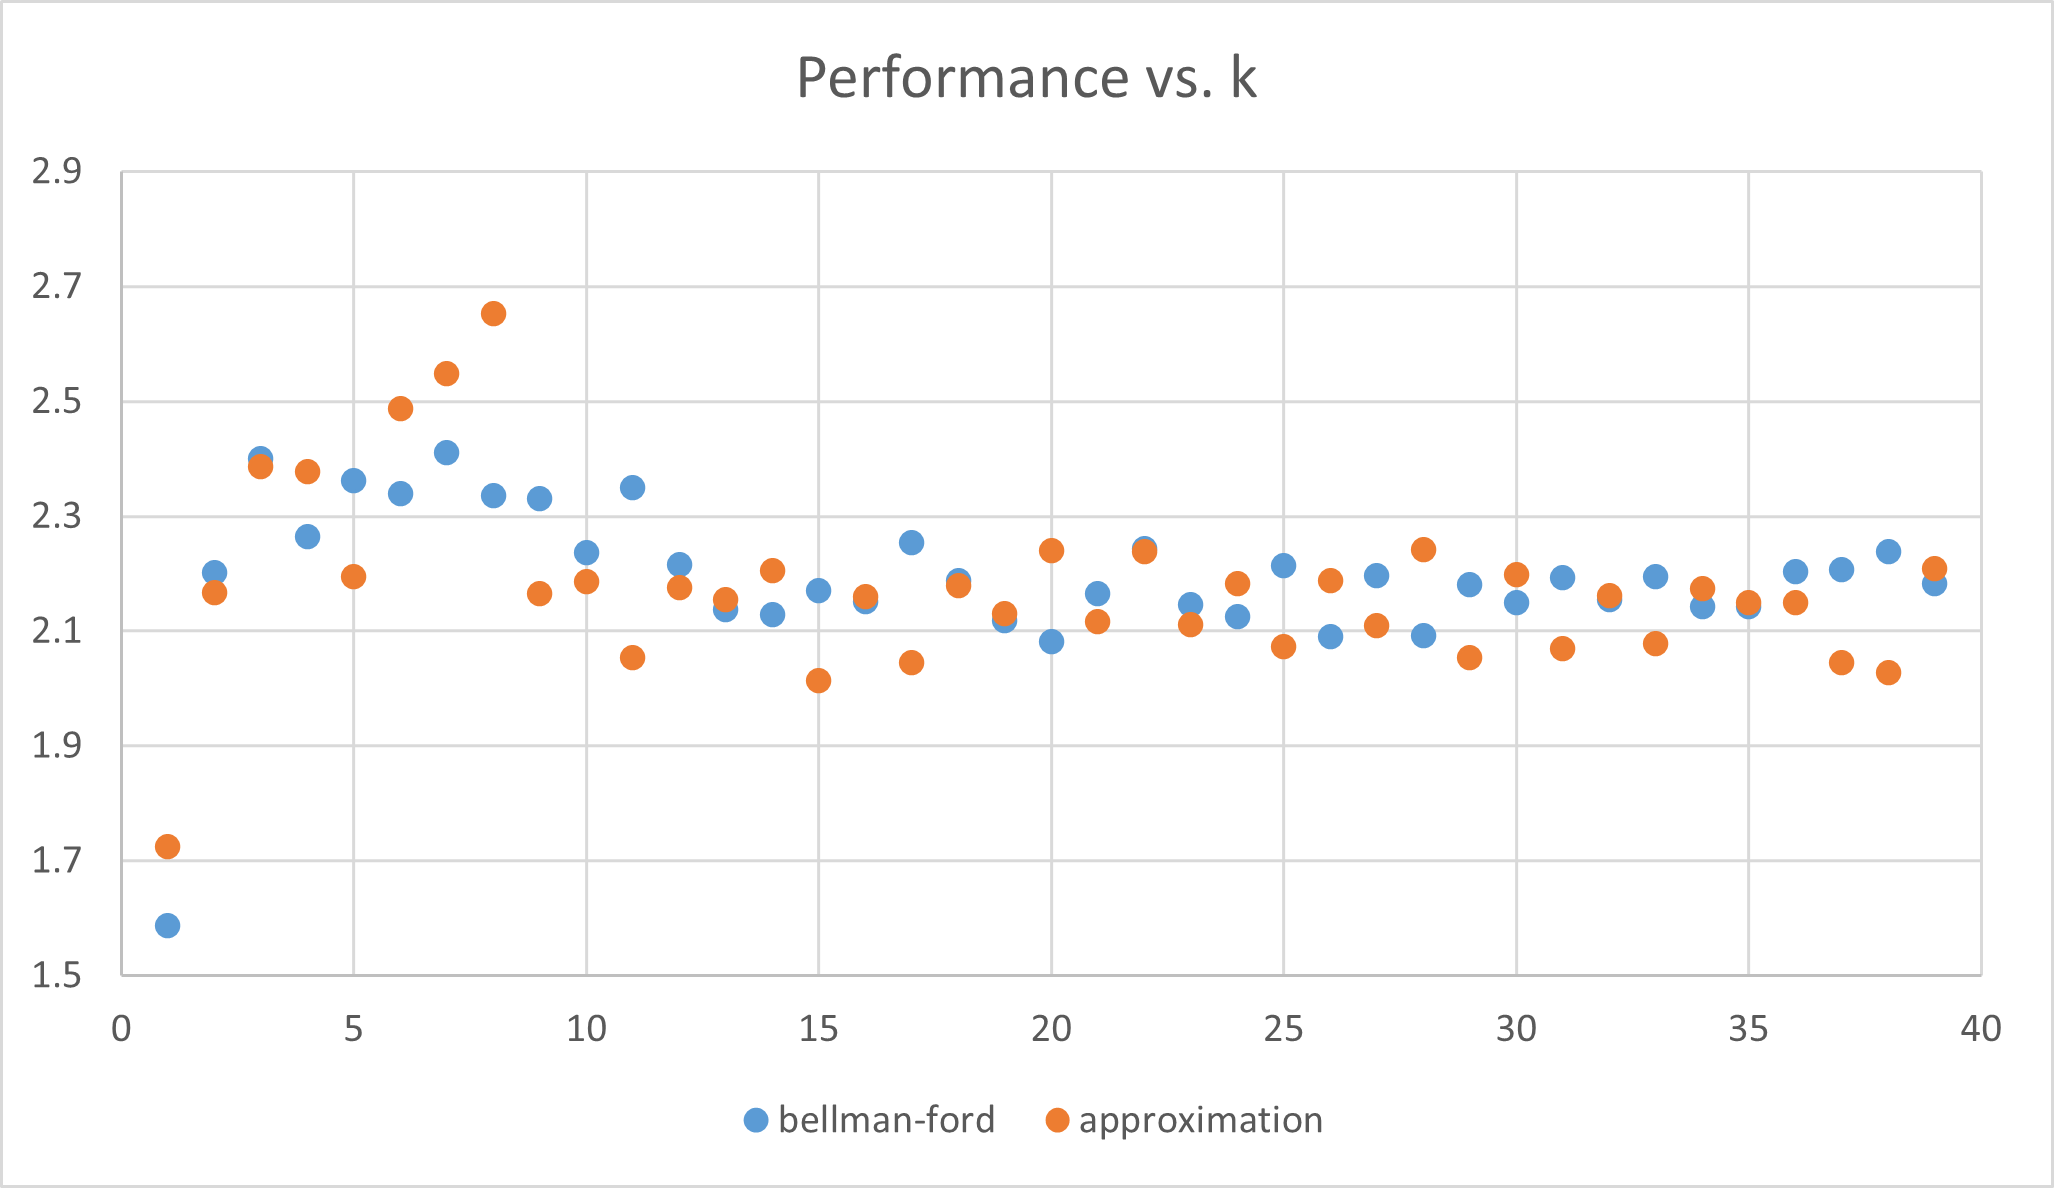
\includegraphics[width=0.7\textwidth,height=\textheight,keepaspectratio]{bellman_ford_time.png}
\caption{performance of bellman-ford and an approximation vs. k}
\label{Figure: m1}
\end{figure}
\noindent The timing data we collected doesn't show any clear correlation between $k$ and performance. In fact, some trials resulted in the approximation performing worse than the original algorithm, which seems erroneous. This may be due to the additional overhead in our approximation algorithm. That algorithm updates each element of an array of length $n$ up to $k$ times, which can be expensive as $n$ becomes large. Our approximation generally seems to terminate slightly before the original algorithm does, but this improvement in performance is negligible compared to the imprecision of the data.\\
We expect the total distance to each node to become more accurate as $k$ increases, with low $k$ values resulting in the approximation overestimating the total distance. This is because \verb-dist[neighbour] = dist[node] + G.w(node, neighbour)- is only run when the algorithm finds a shorter path to a node. If we restrict this process with $k$, the shortest distance to a specific node might not be found. The total distance to each node (or the minimum spanning tree) is shown in the chart below.
\begin{figure}[H]
\centering
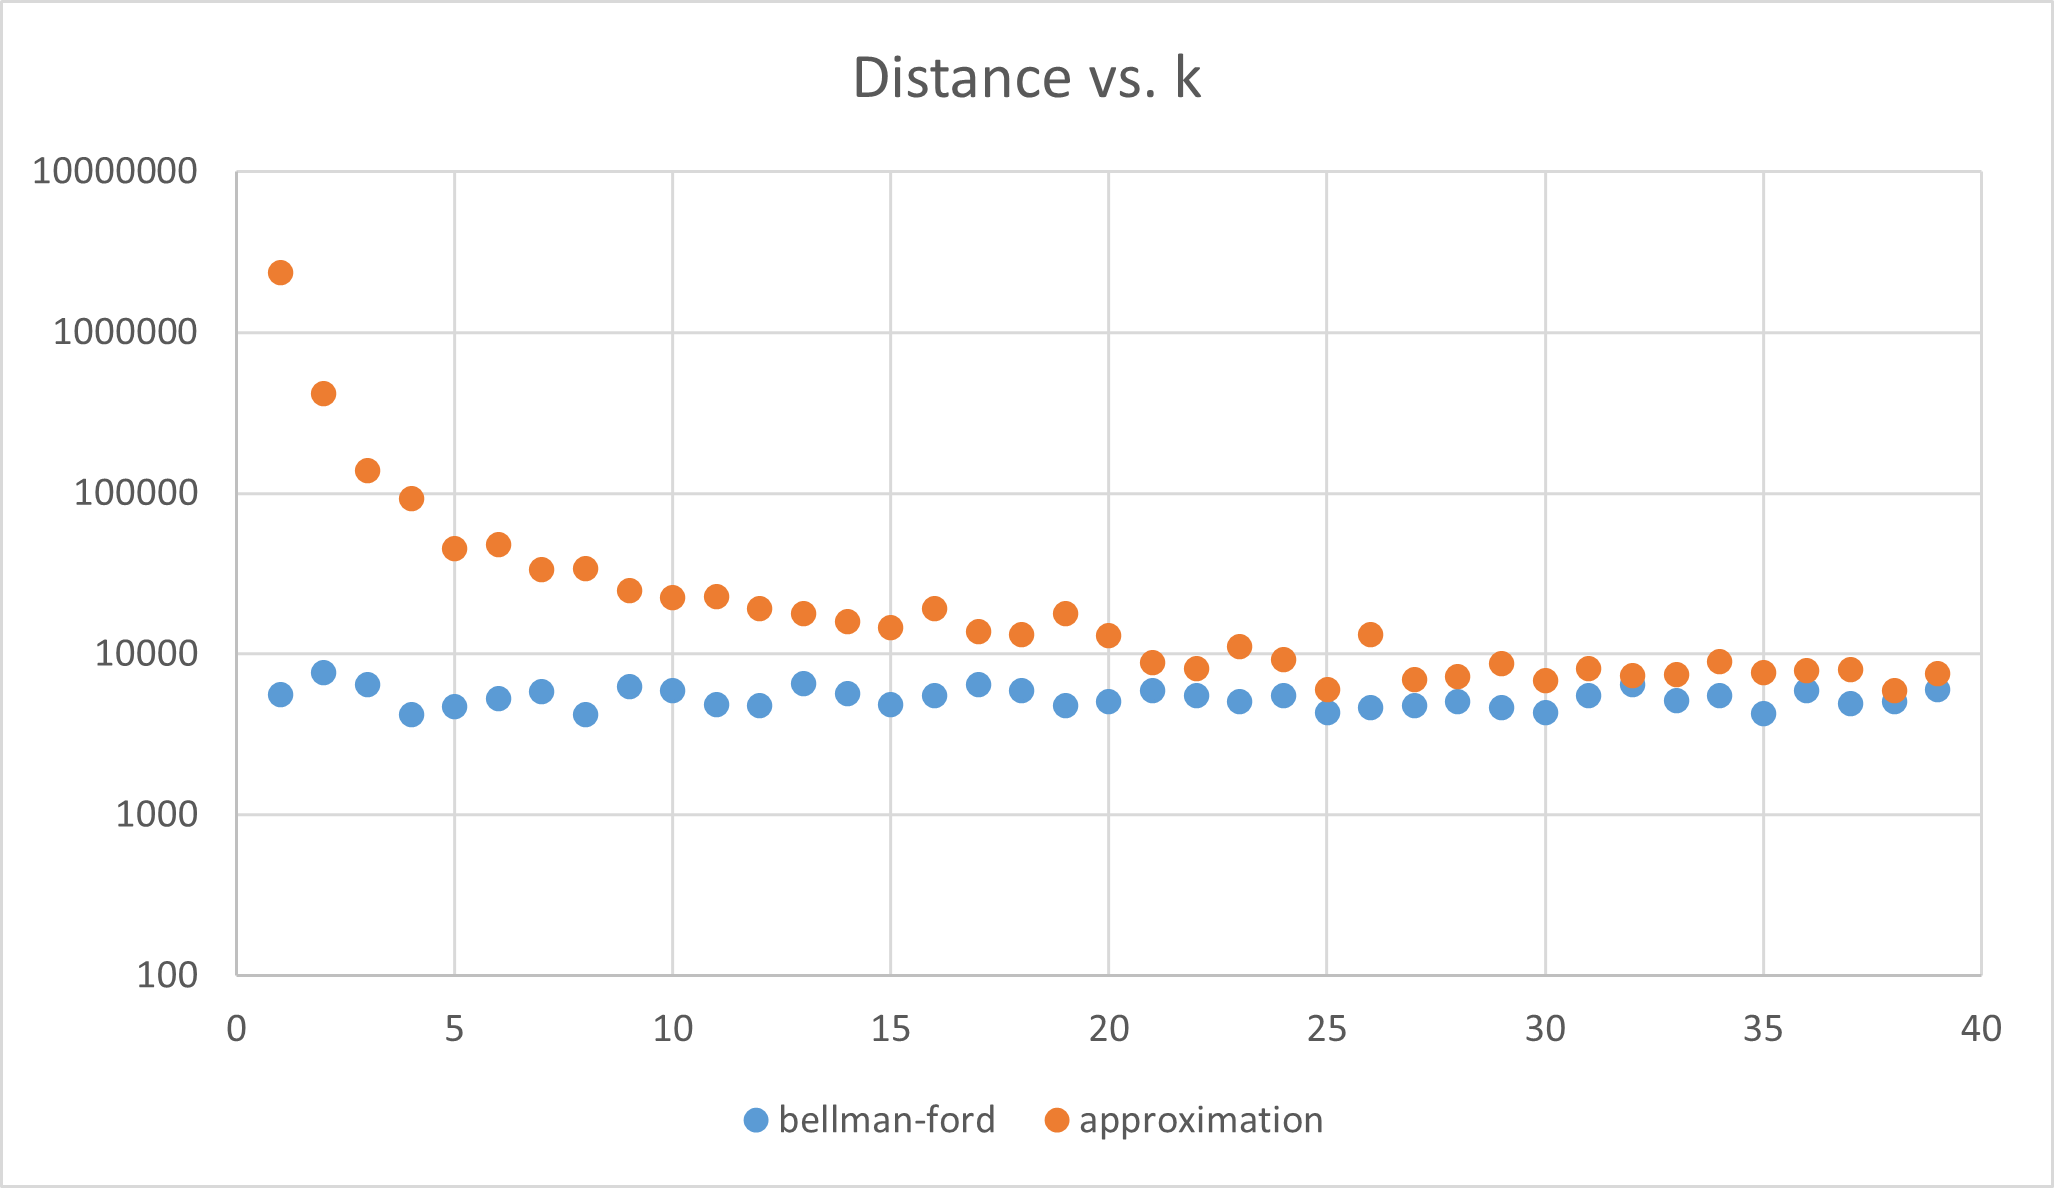
\includegraphics[width=0.7\textwidth,height=\textheight,keepaspectratio]{bellman_ford_dist.png}
\caption{total distance calculated by bellman-ford and an approximation vs. k}
\label{Figure: m2}
\end{figure}
Our approximated Bellman-Ford performed as expected. For low $k$ values, the approximate total distance was much higher than the distance calculated by the original method. Around $k=20$, the approximate and actual total distances converge. We would recommend a $k$ value above 20 because that is when the error made by the approximated distance becomes reasonably small. Our timing data does not suggest that a specific value of $k$ is better for performance. 

\subsection{All Pairs}
Our implementations for \verb+all_pairs_dijkstra()+ and \verb+all_pairs_bellman_ford()+ use the same approach as the algorithms given in \verb+lab9.py+. To make each algorithm find the shortest path from every node to every other node of a graph, we compute the array of distances from a source node to every other node for each node in the graph using \verb+dijkstra()+ and \verb+bellman_ford()+ respectively. Since Dijkstra has complexity $O(V^2)$ for dense graphs and Bellman-Ford has $O(V^3)$
for dense graphs, I would expect the all-pairs versions of these algorithms to have $O(V^3)$ and $O(V^4)$ complexities. This is because they consist of running Dijkstra and Bellman-Ford $V$ times and $O(V)\times O(V^2)=O(V^3)$, $O(V)\times O(V^3)=O(V^4)$.
\subsection{Mystery}
The \verb+mystery()+ function in \verb+lab9.py+ uses a helper function \verb+init_d()+ that takes in a graph and initializes the shortest distance matrix. For each path from node $i$ to node $j$, the function checks if these nodes are connected. If they are connected, then the matrix entry for \verb+d[i][j]+ is assigned the weight of the edge between them. Otherwise, it is assigned 999999. The \verb+mystery()+ function iterates through each node $V^2$ times. It checks if the recorded path from some node $i$ to $j$ is greater than the sum of the paths from $i$ to another node $k$ and $k$ to $j$. If so, the shortest path distance is updated. After some testing, we concluded that \verb+mystery()+ does not work on graphs with negative edge weights. We ran some experiments on \verb+mystery()+ and \verb+all_pairs_dijkstra()+ and \verb+all_pairs_bellman_ford()+ to see how they perform. We used the same method as in the Bellman-Ford Approximation, except we chose to vary $V$, the number of nodes instead of $k$. We still tested these algorithms on connected graphs with positive edge weights. First, we verified that all three algorithms output the same path matrix when given the same graph. Then we tested the time each algorithm takes to generate the path matrix when given the same graph. We conducted our tests on graphs with $V$ ranging from 1 to 40. The results are shown in the chart below.
\begin{figure}[H]
\centering
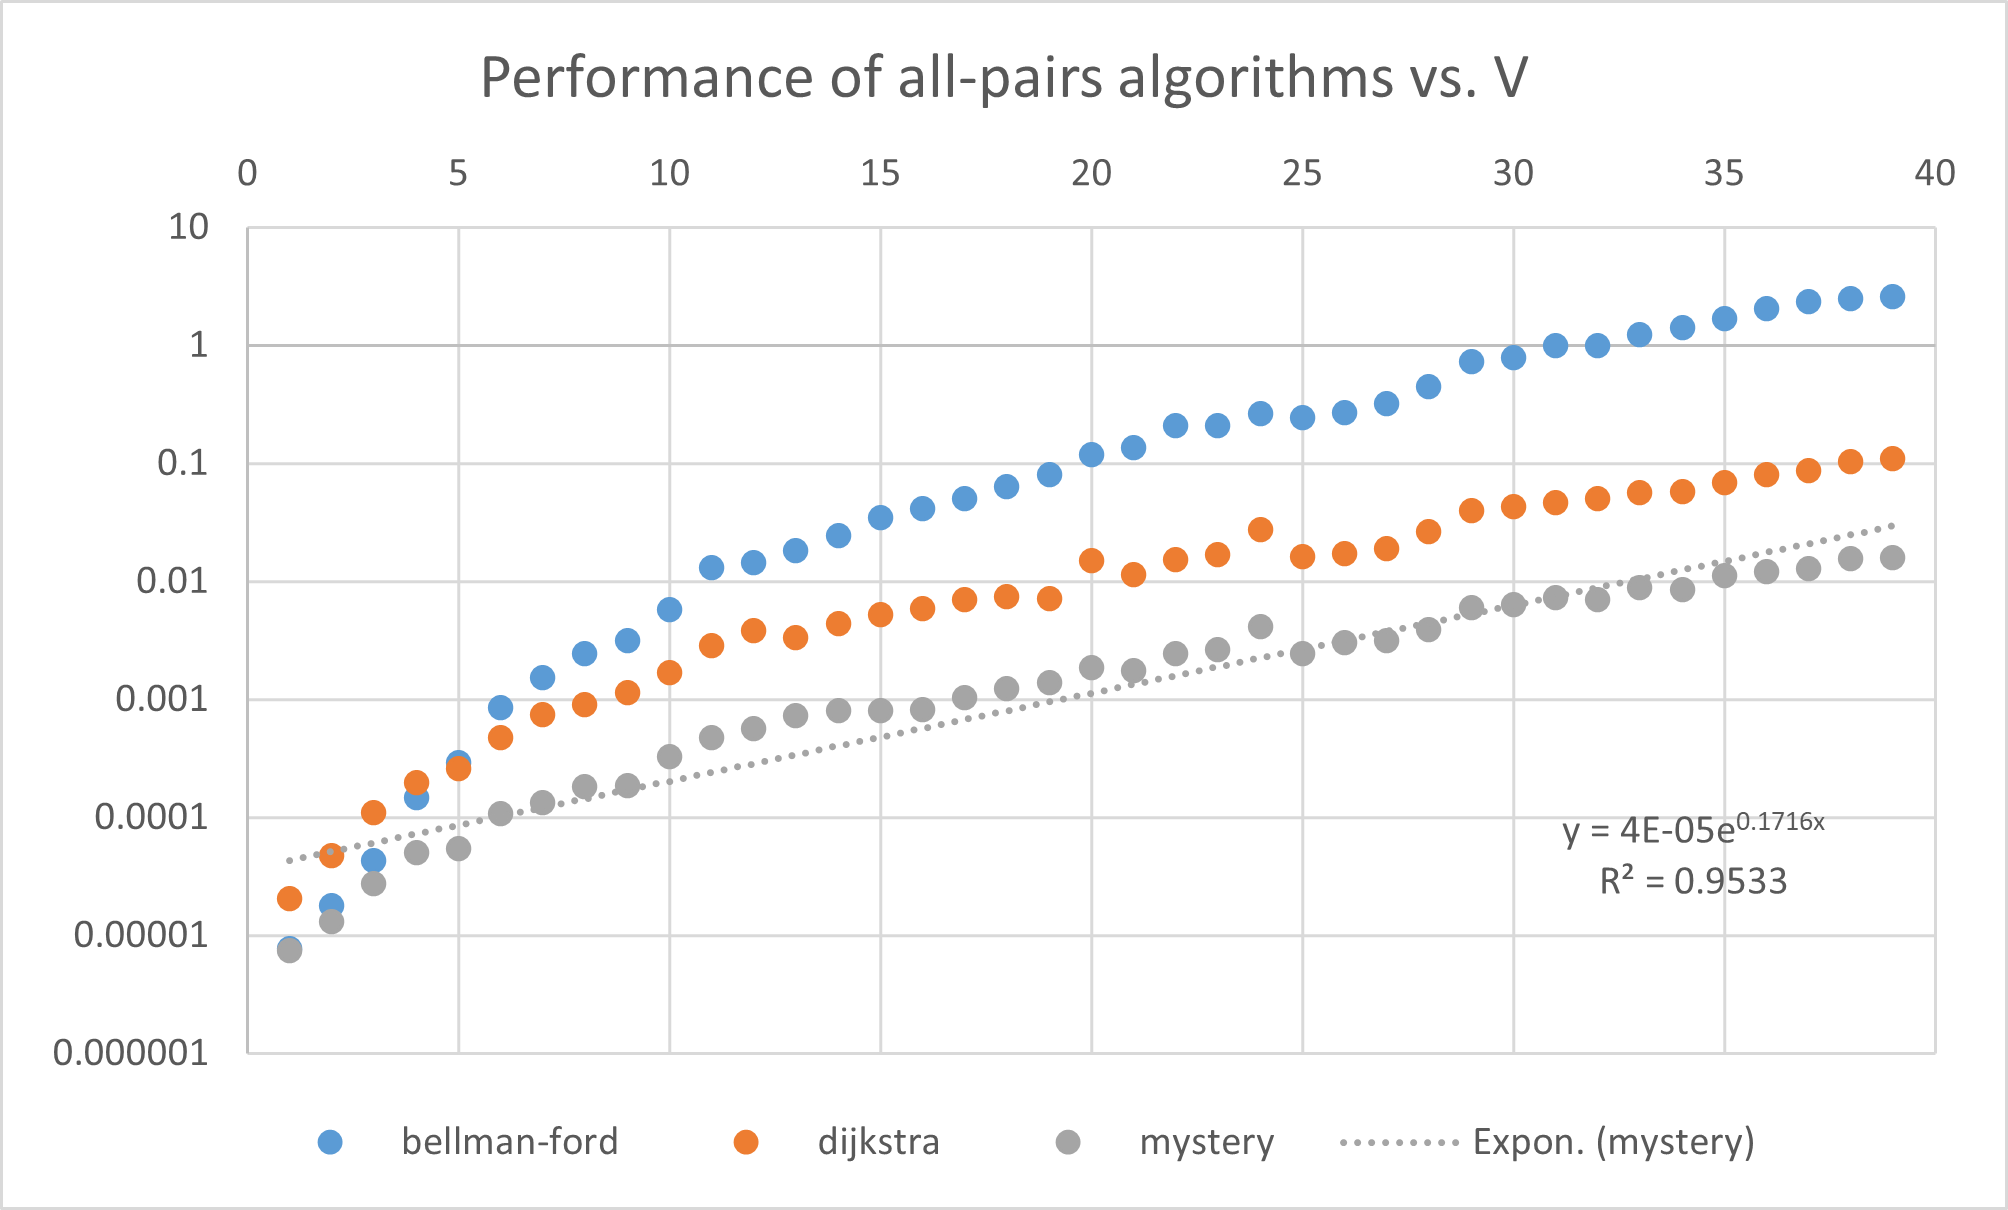
\includegraphics[width=0.7\textwidth,height=\textheight,keepaspectratio]{mystery.png}
\caption{performance of mystery function vs. V}
\label{Figure: m3}
\end{figure}
\noindent It is clear from the structure of the code that \verb+mystery()+ has time complexity $O(V^3)$, similar to \verb+all_pairs_dijkstra()+. That is why its performance in our experiments is surprising. \verb+mystery()+ runs much faster than \verb+all_pairs_dijkstra()+ despite its simple implementation and data structures. From the graph, we can see that \verb+mystery()+ exhibits similar asymptotic behaviours to \verb+all_pairs_dijkstra()+. However, it is consistently faster. This implies that \verb+all_pairs_dijkstra()+ may have more overhead. This makes sense because Dijkstra makes use of dictionaries and a min heap, while the mystery algorithm only maintains a single, 2-dimensional list.


\end{document}

